\documentclass[a4paper,5pt]{amsbook}
%%%%%%%%%%%%%%%%%%%%%%%%%%%%%%%%%%%%%%%%%%%%%%%%%%%%%%%%%%%%%%%%%%%%%

\usepackage{booktabs}
\usepackage{graphicx}
\usepackage{multicol}
\usepackage{textcomp}
\usepackage{systeme}
\usepackage{amssymb}
\usepackage[]{amsmath}
\usepackage{subcaption}
\usepackage[inline]{enumitem}
\usepackage{gensymb}

%%%%%%%%%%%%%%%%%%%%%%%%%%%%%%%%%%%%%%%%%%%%%%%%%%%%%%%%%%%%%%

\newcommand{\sen}{\,\mbox{sen}}
\newcommand{\tg}{\,\mbox{tg}\,}
\newcommand{\cosec}{\,\mbox{cosec}\,}
\newcommand{\cotg}{\,\mbox{cotg}\,}
\newcommand{\tr}{\,\mbox{tr}\,}
\newcommand{\ds}{\displaystyle}
\newcommand{\ra}{\rightarrow}

%%%%%%%%%%%%%%%%%%%%%%%%%%%%%%%%%%%%%%%%%%%%%%%%%%%%%%%%%%%%%%%%%%%%%%%%

\setlength{\textwidth}{16cm} \setlength{\topmargin}{-1.7cm}
\setlength{\textheight}{25cm}
\setlength{\leftmargin}{1.2cm} \setlength{\rightmargin}{1.2cm}
\setlength{\oddsidemargin}{0cm}\setlength{\evensidemargin}{0cm}

%%%%%%%%%%%%%%%%%%%%%%%%%%%%%%%%%%%%%%%%%%%%%%%%%%%%%%%%%%%%%%%%%%%%%%%%

% \renewcommand{\baselinestretch}{1.6}
% \renewcommand{\thefootnote}{\fnsymbol{footnote}}
% \renewcommand{\theequation}{\thesection.\arabic{equation}}
% \setlength{\voffset}{-50pt}
% \numberwithin{equation}{chapter}

%%%%%%%%%%%%%%%%%%%%%%%%%%%%%%%%%%%%%%%%%%%%%%%%%%%%%%%%%%%%%%%%%%%%%%%

\begin{document}
\thispagestyle{empty}
\pagestyle{empty}
\begin{minipage}[h]{0.14\textwidth}
	
\includegraphics[scale=0.24]{../ufgd.png}
\end{minipage}
\begin{minipage}[h]{\textwidth}
\begin{tabular}{c}
{{\bf UNIVERSIDADE FEDERAL DA GRANDE DOURADOS}}\\
{{\bf C\'alculo Diferencial e Integral --- Lista 5}}\\
{{\bf Prof.\ Adriano Barbosa}}\\
\end{tabular}
\vspace{-0.45cm}
%
\end{minipage}

%------------------------

\vspace{1cm}
%%%%%%%%%%%%%%%%%%%%%%%%%%%%%%%%   formulario  inicio  %%%%%%%%%%%%%%%%%%%%%%%%%%%%%%%%
\begin{enumerate}
    \vspace{0.5cm}
    \item Determine em quais intervalos a fun\c{c}\~ao abaixo \'e cont\'{\i}nua.
        \begin{figure}[h]
            \centering
            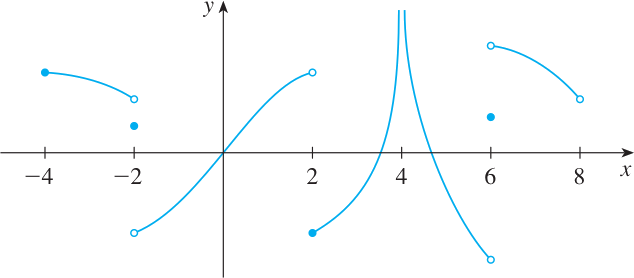
\includegraphics[width=0.5\textwidth]{lista-05-fig1.png}
        \end{figure}

    \vspace{0.5cm}
    \item Usando a defini\c{c}\~ao de continuidade e as propriedades de limite,
        determine se as fun\c{c}\~oes abaixo s\~ao cont\'{\i}nuas nos pontos dados:
        \begin{enumerate}
            \vspace{0.3cm}
            \item $f(x)=3x^4-5x+\sqrt[3]{x^2+4}$, $a=2$
            \vspace{0.3cm}
            \item $f(x)={(x+2x^3)}^4$, $a=-1$
            \vspace{0.3cm}
            \item $f(x)=\ds\frac{2x-3x^2}{1+x^3}$, $a=1$
            % \vspace{0.3cm}
            % \item $f(x)=\left\{
            %         \begin{array}{rl}
            %             \cos(x), & \text{ se } x<0 \\
            %             0, & \text{ se } x=0 \\
            %             1-x^2, & \text{ se } x>0
            %         \end{array}\right.$, $a=0$
        \end{enumerate}

    \vspace{0.5cm}
    \item Use os teoremas sobre fun\c{c}\~oes cont\'{\i}nuas e explique porque as
        fun\c{c}\~oes abaixo s\~ao cont\'{\i}nuas em todos os pontos do seu dom\'{\i}nio:
        \begin{enumerate}
            \vspace{0.3cm}
            \item $F(x)=\ds\frac{2x^2-x-1}{x^2+1}$
            \vspace{0.3cm}
            \item $h(x)=\ds\frac{\sen(x)}{x+1}$
            \vspace{0.3cm}
            \item $g(x)=\cos(1-x^2)$
            \vspace{0.3cm}
            \item $f(x)=\sen(\cos(\sen(x)))$
        \end{enumerate}

    \vspace{0.5cm}
    \item Determine o valor de $f(2)$ de modo que a fun\c{c}\~ao
        $f(x)=\ds\frac{x^3-8}{x^2-4}$ seja cont\'{\i}nua em $2$.

    \vspace{0.5cm}
    \item Sejam $f$ e $g$ cont\'{\i}nuas em $2$, $g(2)=6$ e $\ds\lim_{x\ra2}
        \left[3f(x)+f(x)g(x)\right]=36$. Determine o valor de $f(2)$.

    \vspace{0.5cm}
    \item Use a continuidade das fun\c{c}\~oes para calcular os limites abaixo:

        \begin{enumerate*}
            \item $\ds\lim_{x\ra4}\frac{5+\sqrt{x}}{\sqrt{5+x}}$
            \hspace{1cm}
            \hspace{1cm}
            \item $\ds\lim_{x\ra\frac{\pi}{4}} x\cos^2(x)$
        \end{enumerate*}

    \vspace{0.5cm}
    \item Use o Teorema do Valor Intermedi\'ario para mostrar que existe uma
        raiz das equa\c{c}\~oes abaixo no intervalo dado:

        \begin{enumerate*}
            \item $x^4+x-3=0$, $(1,2)$
            \hspace{0.5cm}
            \hspace{0.5cm}
            \item $\cos(x)=x$, $(0,1)$
            \hspace{0.5cm}
            \hspace{0.5cm}
            \item $\sen(x)=x^2-x$, $(1,2)$
        \end{enumerate*}
\end{enumerate}

\end{document}
